\documentclass[12pt, a4paper]{report}
\usepackage{graphicx}
\usepackage[brazilian]{babel}
\usepackage[utf8x]{inputenc}
\usepackage{setspace}
\usepackage{hyperref}
\usepackage[small,bf]{caption}
\usepackage{amsmath, amssymb, pxfonts}
\usepackage{textcomp}
\usepackage{nomencl}
\makenomenclature
\usepackage{longtable}
\usepackage{tikz}
\usepackage{mathrsfs}
\everymath{\displaystyle}
\usepackage{natbib}
\usepackage{emptypage}
%\usepackage{fancyhdr}
\usepackage{lastpage}

\usepackage{nopageno}

%%%%%%%%%%%%%%%%%%%%%%%%%%%%%%%%%%%%%%%%%%%%%%%%%%%%%%%%%%%%%%%%%%%%
%%%
%%% Macros 
%%% Curso de Especialização em Sistemas Eletrônicos para Controle
%%% Faculdade SENAI Anchieta - São Paulo - SP
%%% José William Rodrigues Pereira 
%%% Outubro / 2015
%%%
%%%%%%%%%%%%%%%%%%%%%%%%%%%%%%%%%%%%%%%%%%%%%%%%%%%%%%%%%%%%%%%%%%%%

%%%------------------------------------ Dados
\def\autor#1{\gdef\autor{#1}}
\def\nome#1{\gdef\nome{#1}}
\def\ultimonome#1{\gdef\ultimonome{#1}}
\def\titulo#1{\gdef\titulo{#1}}
\def\subtitulo#1{\gdef\subtitulo{#1}}
\def\curso#1{\gdef\curso{#1}}
\def\instituicao#1{\gdef\instituicao{#1}}
\def\sigla#1{\gdef\sigla{#1}}
\def\unidadeacademica#1{\gdef\unidadeacademica{#1}}
\def\grau#1{\gdef\grau{#1}}
\def\tipodotrabalho#1{\gdef\tipodotrabalho{#1}}
\def\orientador#1{\gdef\orientador{#1}}
\def\torientador#1{\gdef\torientador{#1}}
\def\coorientador#1{\gdef\coorientador{#1}}
\def\tcoorientador#1{\gdef\tcoorientador{#1}}
\def\cidade#1{\gdef\cidade{#1}}
\def\ano#1{\gdef\ano{#1}}
\def\npaginas#1{\gdef\npaginas{#1}}
\def\CDU#1{\gdef\CDU{#1}}
\def\areas#1{\gdef\areas{#1}}
\def\examinadorum#1{\gdef\examinadorum{#1}}
\def\texaminadorum#1{\gdef\texaminadorum{#1}}
\def\examinadordois#1{\gdef\examinadordois{#1}}
\def\texaminadordois#1{\gdef\texaminadordois{#1}}
\def\data#1{\gdef\data{#1}}
\def\palavraschave#1{\gdef\palavraschave{#1}}
\def\keywords#1{\gdef\keywords{#1}}

%%%%------------------------------------ Configuração das Páginas
\newcommand{\configuramargens} %%% Define margens
{
  \usepackage[width=210.00mm, height=297.00mm, 
			  left=3.00cm,    right=2.00cm, 
			  top=3.00cm,     bottom=2.00cm] {geometry}
}

%%%------------------------------------ Fonte
\renewcommand{\familydefault}{\sfdefault} % sans font
%\renewcommand{\familydefault}{\rmdefault}  % roman font


%%%------------------------------------ Formatação de Capitulo
\titleformat{\chapter}
  {\Large\bfseries}
  {}
  {0pt}
  {\huge}

%%%------------------------------------ Capa
\newcommand{\capa}
{
  \begin{titlepage}
    \thispagestyle{empty}
    \begin{center}
      \textsc{\instituicao} 		\\[0.0cm]
      \textsc{\unidadeacademica}	\\[0.0cm]
      \textsc{Curso de \curso}		\\[4.0cm]
      \textsc{\autor}			\\[4.0cm]
      \textsc{\titulo}			\\[0.0cm]
      \textsc{\subtitulo}               \\[0.4cm]
      \vfill
      \textsc{\cidade}			\\[0.0cm]
      \textsc{\ano}			\\[0.0cm]
    \end{center}
  \end{titlepage}
}
%%%------------------------------------ Natureza
\newcommand{\natureza}
{
  \begin{flushright}
    \thispagestyle{empty}
    \begin{minipage}{0.5\textwidth}
    {
      \tipodotrabalho apresentada à \instituicao 
      como requisito para   obtenção do grau de \grau em \curso
    } 				\\[0.4cm]
    Orientador:   \torientador    \orientador \\
    Coorientador: \tcoorientador  \coorientador
    \end{minipage}
  \end{flushright}
}
%%%------------------------------------ Folha de Rosto
\newcommand{\folhaderosto}
{
  \begin{titlepage}
    \begin{center}
      \textsc{ }		\\[4.0cm]
      \textsc{\autor}		\\[4.0cm]
      \textsc{\titulo}		\\[0.0cm]
      \textsc{\subtitulo}       \\[4.0cm]
      \natureza
      \vfill
      \textsc{\cidade}		\\[0.0cm]
      \textsc{\ano}		\\[0.0cm]
    \end{center}
  \end{titlepage}
}
%%%------------------------------------ Ficha Catalográfica
\newcommand{\fichacatalografica}
{
  \begin{titlepage}
    \vfil\null
    \vfill
    \fbox
    {
      \begin{tabular}{p{13.0cm}}
        \ultimonome, \nome                      \\
        \titulo \subtitulo\ / \nome\ \ultimonome\ -  \ano \\
        \npaginas .p                \\
        \areas . I.Título. \\
        \hfill CDU \CDU
      \end{tabular} 
    }  
 \end{titlepage}
}
%%%------------------------------------ Folha de Aprovação
\newcommand{\folhadeaprovacao}
{
  \begin{titlepage}
    \thispagestyle{empty}
    \begin{center}
      \textsc{\autor}
      \vfill
      \textsc{ \titulo } \\
      \textsc{ \subtitulo }
      \vfill
    \end{center}
    \natureza
    \vfill
    \centering Aprovado pela banca examinadora em \data \\
    \vfill
    \begin{center}
      {\large\bfseries BANCA EXAMINADORA }\\
      \vfill
      \rule{9.0cm}{0.1mm} \\
      {\torientador \orientador  }\\
      {Orientador } \\
      \vfill
      \rule{9.0cm}{0.1mm} \\
      {\tcoorientador \coorientador} \\
      {Coorientador} \\
      \vfill
      \rule{9.0cm}{0.1mm} \\
      {\texaminadorum \examinadorum }\\
      \vfill
      \rule{9.0cm}{0.1mm} \\
      {\texaminadordois \examinadordois}
    \end{center}
  \end{titlepage}
}
%%%------------------------------------ Dedicatória
\newcommand{\dedicatoria}[1]
{
  \begin{titlepage}
  \thispagestyle{empty}
  \hspace{1cm}
  \vfill
  \begin{flushright}
    \begin{minipage}{0.6\textwidth}
    \textrm
    {
      \textit
      {
	#1
      }
    }    
    \end{minipage}
  \end{flushright}
  \end{titlepage}
}

%%%------------------------------------ Agradecimentos
\newcommand{\agradecimentos}[1]
{
  \begin{titlepage} 
    \thispagestyle{empty}
    \titlepage
    \begin{center}%
        \huge \textbf{Agradecimentos}
    \end{center}%
    \null
    \hspace{1cm} #1
    \endtitlepage
  \end{titlepage}
}

%%%------------------------------------ Epígrafe
\newcommand{\epigrafe}[1]
{
  \begin{titlepage}
    \thispagestyle{empty} 
    \hspace{1cm}
    \vfill
    \begin{flushright}
      \begin{minipage}{0.6\textwidth}
      \textrm
      {
        \textit
        {
	    #1
        }
      }    
      \end{minipage}
    \end{flushright}
  \end{titlepage}
}

%%%------------------------------------ Resumo
\newcommand{\resumo}[1]
{
  \begin{titlepage} 
    \titlepage  
    \thispagestyle{empty}
    \begin{center}%
        \huge \textbf{Resumo}
    \end{center}%
    \null
    #1

    \textbf{\\PALAVRAS-CHAVE:} \palavraschave
    \endtitlepage
  \end{titlepage}
}
%-------------------------------------- Abstract
\newcommand{\resumolinguaestrangeira}[1]
{
  \begin{titlepage} 
    \titlepage
    \thispagestyle{empty}  
    \begin{center}%
        \huge \textbf{Abstract}
    \end{center}%
    \null
    \hspace{1cm} #1

    \textbf{\\KEYWORDS:} \keywords
    \endtitlepage
  \end{titlepage}
}
%-------------------------------------- Sumário
\newcommand{\sumario}
{
    \tableofcontents
    \thispagestyle{empty}
}
%-------------------------------------- Lista de figuras
\newcommand{\listadefiguras}
{
  \listoffigures
  \thispagestyle{empty}
}
%-------------------------------------- Lista de tabelas
\newcommand{\listadetabelas}
{
  \listoftables
  \thispagestyle{empty}
}

%-------------------------------------- Lista de abreviaturas e siglas
\newcommand{\abreviatura}[2]
{
  \nomenclature{#1}{#2}
  #1
}
\newcommand{\listadeabreviaturasesiglas}
{
  \renewcommand{\nomname}{Lista de abreviaturas e siglas}
  \printnomenclature[5em]
  \thispagestyle{empty}	
}
%%%------------------------------------ Citação
\newcommand{\citacao}[1]
{
  \begin{flushright}
    \begin{minipage}{12cm}
      \footnotesize #1
    \end{minipage}
    \vspace{12pt}
  \end{flushright}
}

%--------------------------------------
%--------------------------------------


%--------------------------------------
%-------------- Estilo do Codigo Fonte
\definecolor{verde}{rgb}{0.25,0.5,0.35}
\definecolor{jpurple}{rgb}{0.5,0,0.36}

\lstset{
  language=C,
  basicstyle=\ttfamily\small,
  keywordstyle=\color{blue},
  stringstyle=\color{verde},
  commentstyle=\color{red},
  extendedchars=true,
  showspaces=false,
  showstringspaces=false,
  numbers=left,
  numberstyle=\small,
  breaklines=true,
  backgroundcolor=\color{green!10},
  breakautoindent=true,
  captionpos=b,
  xleftmargin=0pt,
}

%--------------------------------------:w





%%%----------------------------------- Declarações
\autor{JOSÉ WILLIAM RODRIGUES PEREIRA}
\nome{José William Rodrigues }
\ultimonome{Pereira}
\titulo{ ESTUDO COMPARATIVO ENTRE TÉCNICAS DE CONTROLE:}
\subtitulo{ PID e LÓGICA PARACONSISTENTE}
\curso{Sistemas Eletrônicos para Controle }
\instituicao{Faculdade de Tecnologia SENAI Anchieta }
\sigla{FTSA }
\unidadeacademica{Pós-Graduação Lato Sensu }
\grau{Especialista }
\tipodotrabalho{Monografia } 
\orientador{Vander Celio Nunes }
\torientador{Profº Me.}
\coorientador{Rudson de Lima Silva}
\tcoorientador{Profº Me. }
\cidade{São Paulo}
\ano{2016}
\npaginas{\pageref{LastPage}}
\CDU{xxx.yy}
\areas{	1.Técnicas de Controle 
	2.Lógica Paraconsistente
	3.Controle PID Digital}
\examinadorum{ Marcos Antônio Felizola}
\texaminadorum{Profº Me.}
\examinadordois{ José Gil de Oliveira}
\texaminadordois{Profº Me.}
\data{dd/mm/aaaa}
%%%%%%%%%%%%%%%%%%%%%%%%%%%%%%%%%%%%%%%%
%%%% Inicio do documento
%%%%%%%%%%%%%%%%%%%%%%%%%%%%%%%%%%%%%%%%
\configuramargens

\begin{document}
\capa
\folhaderosto
\fichacatalografica
\folhadeaprovacao

\dedicatoria{      Dedico este trabalho à minha família, 
      pela paciência;
      aos amigos de curso e professores, 
      pelo companheirismo e dedicação;
      a todos que em algum momento compartilharam 
      ideias, palavras de incentivo e carinho;
      A todos os amantes do saber.
}
\agradecimentos{À minha família e à minha noiva Fernanda, que além de apoio incondicional souberam compreender todo o esforço e dedicação destinados a este estudo.

Ao Profº Me. Vander Célio Nunes por apresentar e ensinar a Lógica Paraconsistente Anotada Com Anotação de Dois Valore (LPA2v), pela dedicação e orientação ao longo do curso e sempre que precisei.

Ao Profº Me. Rudson de Lima Silva pela dedicação nas aulas e na coorientação, pelo respeito ao conhecimento e pela paixão pela docência, certamente um dos pilares que orientam minha carreira docente.

Ao Profº Engº Erineu Claudemir Bellini pela dedicação e pelo amor ao saber, por servir de exemplo e inspiração desde os tempos de curso técnico nesta mesma instituição uma década atrás, talvez o primeiro farol em que me orientei quando tornei-me instrutor, e tive a oportunidade de perceber com alegria o quanto fui influenciado. 

Ao Profº Me. Leandro Poloni Dantas pela qualidade e notório conhecimento na área de sistemas microcontrolados, objetivo principal pelo qual busquei este curso de especialização, que superou em muito minhas espectativas.

Ao Serviço Nacional de Aprendizagem Industrial (SENAI) de São Paulo, onde ministro aulas como Instrutor de Formação Profissional na área de eletrônica aos cursos de aprendizagem industrial e técnico em eletroeletrônica, pela bolsa de estudos concedida sob aprovação do senhor diretor Profº Me. Carlos Alberto Gomes da unidade SENAI "Frederico Jacob" no Tatuapé e também ao senhor diretor Profº Augusto Lins de Albuquerque Neto, da Faculdade de Tecnologia SENAI Anchieta, coordenadores, professores e demais funcionários dessa unidade, um destaque ao Coordenador Profº Me. Marcos Antônio Felizola que sempre esteve disposto a dialogar e dirimir eventuais problemas e dificuldades.

À todos os colegas que fizeram parte desta jornada algo agradável e divertido, mostrando a individualidade e o potencial de cada um, ampliando a noção de respeito, parceria e amizade. 

 
}
\epigrafe{{"... Reze e trabalhe, fazendo de conta que esta vida é um dia de capina 
com sol quente, que às vezes custa muito a passar, mas sempre passa. 
E você ainda pode ter muito pedaço bom de alegria... 
Cada um tem a sua hora e a sua vez: você há de ter a sua." (Sagarana)
}
{
\\
\\
\textbf{ João Guimarães Rosa } 
}}
\resumo{%CONTEXTO: Identifica a grande area de pesquisa e sua importancia;

%LACUNA: (however:contudo, all do:todos fazem) O que precisa ser estudado nesse campo e ainda precisa ser entendido, exclarecido. Local aonde o trabalho está inserido;

%PRÓPOSITO: (this paper describes...)o que foi feito e principal objetivo do artigo;

%METODOLOGIA: Maneira geral falar dos métodos

%RESULTADOS: IMPORTANTÍSSIMO!!! Principal achado, resultado de forma bastante clara;

%CONCLUSOES: Mostrar como que os resutados contribuem para o avanço da grande aréa.

Sistemas de Controle são largamente utilizados principalmente no setor industrial e buscam uma maior eficiência de tempo e energia, mantendo a qualidade dos processos e do sistema controlado, 
% Lacuna
contudo ainda são muito complexos e de difícil implementação, necessitando de um sistema embarcado dedicado.
% Propósito
O objetivo deste estudo é mostrar uma forma alternativa de controle em malha fechada e implementar, um controle não convencional utilizando a Lógica Paraconsistente Anotada com anotação de dois valores (LPA2v), 
% Metodologia
de forma comparativa ao modelo clássico de controle, Proporcional, Integral e Derivativo (PID).
% Resultados
Partindo dos conceitos básicos de controle, o modelo com LPA2v apresenta grande potencial para sua implementação e exploração em sistemas de controle.
%Conclusão		
Comparativamente, o modelo proposto alinha-se ao modelo clássico, tendo parte de sua teoria adaptada para o atendimento dos pressupostos da LPA2v.
		

}
\resumolinguaestrangeira{Abstract}
\listadefiguras
\listadetabelas
\listadeabreviaturasesiglas

\chapter*{Lista de símbolos}
\thispagestyle{empty}
\begin{longtable}[l]{p{50pt} p{200pt}}
  $\lambda $ & grau de evidência \\
\end{longtable}




\sumario

%\singlespacing 	% espaçamento simples
\onehalfspacing		% espaçamento de 1,5
%doublespacing		% espaçamento duplo

\pagestyle{myheadings}
%\pagestyle{fancy}

%\fancyhf{}
%\lhead{\pageref{LastPage}}
%\rhead{\thepage}

\setcounter{page}{0}
\chapter{Introdução}
Comparar sistemas de controle mediante uma mesma planta é uma forma de avaliar as possibilidades e limitações de ambos os elementos de estudo, possibilitando uma melhor escolha no momento de planejar e executar um projeto, obtendo assim um ganho de tempo, que reflete diretamente no custo de implementação e manutenção além de conferir ao projeto maior possibilidade de atingir um melhor desempenho e uma maior confiabilidade. 

Sistemas de controle são largamente utilizados pela indústria como um todo a muitos anos, tendo algumas técnicas amplamente difundidas e com alto grau de maturação, como é o caso do controle Proporcional-Integral-Derivativo (PID),  mesmo apresentando restrições e limitações quanto a aplicação em sistemas que possuem não-linearidades, atrasos de transporte e/ou parâmetros variantes no tempo.\cite{Ferreira2012}

%%%% Estudo Comparativo entre as Técnicas de Controle Fuzzy, PI e Adaptativo Aplicado ao Processo de Fabricação de Papel Reciclado Utilizando a Ferramenta Delta Tune
%%% Cesar Ferreira pag16


Tendo em vista que estudos de novas formas de controle não clássicas estão em curso, a lógica paraconsistente surge como uma promissora ferramenta para implementação de tomada de descisão em diversos campos de aplicação como a robótica, automação industrial, inteligência artificial, logística, controle, entre outras.\cite{JoaoInacio}
 
O presente trabalho tem como objetivo a caracterização de duas teorias utilizadas em sistemas controle, PID e Lógica Paraconsistente Anotada de anotação com dois valores (LPA2v), que é uma das formas de aplicação da Lógica Paraconsistente, sua implementação e posterior comparação utilizando uma plataforma que contemple recursos que possibilite uma análise de desempenho e complexidade de implementação.
%Objetivo ou Finalidade: preocupação em distinguir a característica comum ou as leis gerais que regem determinados eventos.



%%%%%%%%%%%%%%%%%%%%%%%%%%%%%%%%%%%%%%%%%%%%%%%%%%%%%%%%%%%%
\section{Formulação do Problema}
%%%%%%%%%%%%%%%%%%%%%%%%%%%%%%%%%%%%%%%%%%%%%%%%%%%%%%%%%%%%

O cenário dos dispositivos microcontrolados é cada vez maior e abrange uma gama de aplicações muito ampla, desde pequenas aplicações com dispositivos de 8-bits até modernos controladores de 32-bits integrados com hardware dedicado à processamento digital de sinais e cálculos avançados.

A integração de hardware dedicado junto ao núcleo dos microcontroladores, possibilita a implementação de rotinas complexas de cálculo para controle do tipo PID, de forma a dirimir o custo de processamento, intrínseco ao controle clássico, ou seja, a qantidade de ciclos de máquina necessários para a realização dos cálculos e por consequência o tempo de resposta do sistema. 

Em contrapartida, novas técnicas utilizando lógicas modernas, como a LPA2v, possuem baixo custo de processamento em relação aos cálculos matemáticos, por serem inerentemente simples, não necessitando de um hardware dedicado para sua implementação, e podendo ser realizada a execução em dispositivos de menor capacidade de processamento, reduzindo assim o custo do projeto, mas mantendo a qualidade do sinal processado.

Existe a possibilidade de substituir um controlador PID digital por um controlador baseado em lógica paraconsistente, e obter um resultado equivalente em termos de qualidade da resposta do sistema, menor complexidade na codificação de cálculos e carga de processamento reduzida? 

Para responder a essa questão é implementado um sistema com um controlador de 32-bits que possui hardware dedicado, para a comparação entre sistema de controle PID digital e controle baseado em LPA2v.



%%%%%%%%%%%%%%%%%%%%%%%%%%%%%%%%%%%%%%%%%%%%%%%%%%%%%%%%%%%%
\section{Hipótese e Relevância do Trabalho}
%%%%%%%%%%%%%%%%%%%%%%%%%%%%%%%%%%%%%%%%%%%%%%%%%%%%%%%%%%%%

A lógica paraconsistente vem ganhando relevância e adeptos principalmente à partir do final da década de 90 do século XX, quando houve o Primeiro Congresso Mundial sobre Paraconsistência em Gent na Bélgica em 1997, no ano 2000 o segundo congresso realizado em São Sebastião, São Paulo e o terceiro em Toulouse, França em julho de 2003, atraindo cada vez mais pesquisadores interessados de diversos centros de pesquisa do mundo.  \cite{DecioKrause}

Atualmente as pesquisas estão focadas no estudo da aplicação da lógica paraconsistente, e ganhar espaço no universo técnico e científico, contribuindo com uma nova e eficiente forma de trabalho.

Em função da sua simplicidade de implementação, há uma forte expectativa de que possa ser implantada em sistemas embarcados com baixo poder de processamento, como microcontroladores de 8 bits, de forma eficiente, em oposição ao clássico PID de difícil implementação e alto custo de processamento, ou seja, grande quantidade de instruções e maior tempo de resposta em função da complexidade das operações. Assim é de fundamental importância que se faça um estudo comparativo entre as duas técnicas, para que se possa concluir a hipótese de que ambas são equivalentes do ponto de vista da eficiência do controle na planta, mas que do ponto de vista de carga processamento, a lógica paraconsistente é sensivelmente melhor.



%%%%%%%%%%%%%%%%%%%%%%%%%%%%%%%%%%%%%%%%%%%%%%%%%%%%%%%%%%%%
\section{Objetivo Geral}
%%%%%%%%%%%%%%%%%%%%%%%%%%%%%%%%%%%%%%%%%%%%%%%%%%%%%%%%%%%%
%Objeto, subdividido em:
%Material: aquilo que pretende estudar, analisar, interpretar ou verificar de modo geral.
O estudo comparativo entre as técnicas de controle PID-digital e LPA2v, de forma a poder avaliar os sistemas em termos de eficiência do controle, carga de processamento e tempo de resposta.



%%%%%%%%%%%%%%%%%%%%%%%%%%%%%%%%%%%%%%%%%%%%%%%%%%%%%%%%%%%%
\section{Objetivos Específicos}
%%%%%%%%%%%%%%%%%%%%%%%%%%%%%%%%%%%%%%%%%%%%%%%%%%%%%%%%%%%%
%Formal: enfoque especial, em face de diversas ciências que possuem o mesmo objetivo material.
Enfoque especial na comparação e avaliação do comportamento do sistema de controle, nas dificuldades de implementação matemática e decodificação em linguagem C, medição dos tempos de resposta em relação aos estímulos de entrada, na quantidade de memória necessária, precisão e robustez de cada implementação.

Implementar o controle PID-digital utilizando um hardware de alto poder de processamento, e com periféricos dedicados, ou seja, módulo de cálculo para PID nativo. 

Implementar o controle utilizando LPA2v, gerar as funções de controle necessárias utilizando os preceitos da lógica, sendo que não há funções dedicadas à LPA2v nativas ao controlador.

Um enfoque especial é dado à complexidade da implementação no controlador e sua carga de processamento, afim de concluir se é possível uma implementação de baixa capacidade de processamento realizar um controle com precisão comparável ao modo clássico, assim como uma forma híbrida, mesclando a relação capacidade de processamento com precisão do controle. 



%%%%%%%%%%%%%%%%%%%%%%%%%%%%%%%%%%%%%%%%%%%%%%%%%%%%%%%%%%%%
\section{Justificativa}
%%%%%%%%%%%%%%%%%%%%%%%%%%%%%%%%%%%%%%%%%%%%%%%%%%%%%%%%%%%%

%Função: aperfeiçoamento, através de crescente acervo de conhecimento, da relação do homem com o seu mundo.
Sendo o presente trabalho uma análise comparativa entre um sistema de controle clássico e uma lógica moderna para implementar o sistema de controle, sua função primordial é contribuir para a ampliação do conhecimento em uma nova forma de lidar com o mundo, amparado por um saber fortemente enraizado que serve de suporte comparativo à potencial teoria emergente, contribuindo dentro de uma aspecto ainda pouco explorado, mesmo contando com algumas implementações, há escassez de comparações diretas entre as técnicas de controle aqui presentes.



%%%%%%%%%%%%%%%%%%%%%%%%%%%%%%%%%%%%%%%%%%%%%%%%%%%%%%%%%%%%
\section{Limitações da pesquisa}
%%%%%%%%%%%%%%%%%%%%%%%%%%%%%%%%%%%%%%%%%%%%%%%%%%%%%%%%%%%%

%%% Não colocar o elemento TEMPO! 
%%% Colocar até onde vai a pesquisa e o que ela não abordará.

Este trabalho apresenta dois modos de controle, sendo o primeiro um modelo clássico utilizando PID com implementação digital e sintonia de parâmetros pela técnica de Ziegler-Nichols e um segundo modelo utilizando LPA2v, como controle moderno. Não é objetivo do trabalho se aprofundar em questões históricas e nem explorar as diversas técnicas de controle, sintonia ou implementação.

O controlador utilizado possui suporte para implementação de PID, mas não é objetivo mostrar como se configura, ou mesmo abordar lógica de programação e seus fundamentos.



%%%%%%%%%%%%%%%%%%%%%%%%%%%%%%%%%%%%%%%%%%%%%%%%%%%%%%%%%%%%
\section{Estrutura do Trabalho}
%%%%%%%%%%%%%%%%%%%%%%%%%%%%%%%%%%%%%%%%%%%%%%%%%%%%%%%%%%%%




\chapter{Controle de Sistemas}

A palavra \emph{Sistema} tem origem no grego \emph{synístanai} e de acordo com \cite{gramaticaNET} significa "fazer funcionar junto" e uma aplicação precursora do controle é apresentada por Ctesibius de Alexandria ( \cite{encyclopediaBritannica} ) onde um conjunto de reservatórios de água com furo na parte inferior geravam por gotejamento uma marcação do tempo, porém a água do reservatório precisa estar em um nível constante, pois o intervalo de gotejamento é afetado diretamente pela quantidade de água, assim foi criado por Ctesibius um sistema semelhante as boias dos reservatórios atuais para manter o nível de água no reservatório sempre constante.

A modificação do comportamento de um sistema, de forma controlada garantindo uma maior eficiência é o objetivo do controle de sistemas. 

A principal tarefa de um engenheiro, segundo \cite{dorf2011modern} "é o processo de concepção ou invenção de formas, partes e detalhes de um sistema para alcançar um propósito específico", processo este que soma a grande capacidade de análise e a criatividade para atender as demandas da função, como é o caso de projeto em engenharia no segmento de Sistemas de controle, cujo objetivo é obter configuração, especificações e identificação de processos para atender uma necessidade real. Norman S. Nise traz uma concepção semelhante onde "Um sistema de controle consiste em subsistemas e processos(ou plantas) construídos com o objetivo de se obter uma saída desejada com desempenho desejado para uma entrada específica fornecida".

Os sistemas de controle atuam basicamente gerando respostas específicas para estímulos específicos de forma controlada e automática trazendo vantagens nas aplicações de diversas áreas como movimentação de grandes equipamentos com precisão, aplicação em locais remotos ou perigosos, compensação de perturbações, manipulação de dados convenientes etc.



%%%%%%%%%%%%%%%%%%%%%%%%%%%%%%%%%%%%%%%%%%%%%%%%%%%%%%%%%%%%
\section{Diagrama de Blocos}
%%%%%%%%%%%%%%%%%%%%%%%%%%%%%%%%%%%%%%%%%%%%%%%%%%%%%%%%%%%%

Os sistemas de controle são geralmente representados através de diagramas de blocos ou fluxo de sinais, como na Figura \ref{fig:processo} convenientes ao seu desenvolvimento e análise. É composta por uma caixa representando o sistema a ser controlado, setas no sentido da caixa representando as entradas do processo e setas no sentido para fora da caixa para indicar a saída do sistema.

Em um sistema real podem haver muitas variáveis de entrada e de saída, mas a abordagem clássica de controle isola apenas uma das variáveis de entrada e uma de saída, ficando o sistema conhecido pela sigla em inglês SISO (\emph{Single In Single Out} - Única Entrada e Única Saída).

\begin{figure}[!htb]
\centering
\begin{tikzpicture}[scale=1]
%\draw [lightgray](0,0) grid (9,2);
\draw (0,1) -- (3,1);
\draw [black, thick](3,0) rectangle (6, 2) ; 
\draw (6,1) -- (9,1);

\draw [fill](3,1) -- (2.8, 1.1) -- (2.8,0.9) -- (3,1);
\draw [fill](9,1) -- (8.8, 1.1) -- (8.8,0.9) -- (9,1);

\node at (4.5, 1){Sistema};
\node [above] at (1.5,1){Valor de};
\node [below] at (1.5,1){Referência};
\node [above] at (7.5,1){Variável};
\node [below] at (7.5,1){Controlada};
\end{tikzpicture}
\caption{ Diagrama de blocos de sistema de controle}
\label{fig:processo}
\end{figure}


O diagrama de blocos mostrado na Figura \ref{fig:processo} é uma simplificação ao máximo de um sistema de controle, contém apenas o bloco representando o sistema, uma entrada, para o valor de referência, e uma saída com o valor da variável controlada. A Figura \ref{fig:malhaAberta}, divide os bloco do sistema em dois: controlador e planta. Neste caso, um sistema de controle em malha aberta, ou seja, não há uma reinserção do sinal de saída à entrada, chamada de realimentação ou retroalimentação. Assim, a entrada possui o valor de resposta desejada, que alimenta o processo e a saída apresenta a resposta real, porém nada garante que a resposta real está coerente ao valor de entrada.

\begin{figure}[!htb]
\centering
\begin{tikzpicture}[scale=1]
%\draw [lightgray](0,0) grid (15,2);
\draw (0,1) -- (3,1);
\draw [black, thick](3,0) rectangle (6, 2) ; 
\draw (6,1) -- (9,1);
\draw [black, thick](9,0) rectangle (12, 2) ; 
\draw (12,1) -- (15,1);

\draw [fill]( 3,1) -- ( 2.8, 1.1) -- ( 2.8,0.9) -- ( 3,1);
\draw [fill]( 9,1) -- ( 8.8, 1.1) -- ( 8.8,0.9) -- ( 9,1);
\draw [fill](15,1) -- (14.8, 1.1) -- (14.8,0.9) -- (15,1);

\node at ( 4.5, 1){Controlador};
\node at (10.5, 1){Planta};
\node [above] at ( 1.5,1){Valor de};
\node [below] at ( 1.5,1){Referência};
\node [above] at ( 7.5,1){Variável};
\node [below] at ( 7.5,1){Manipulada};
\node [above] at (13.5,1){Variável};
\node [below] at (13.5,1){Controlada};
\end{tikzpicture}
\caption{ Diagrama de blocos de sistema de controle em malha aberta}
\label{fig:malhaAberta}
\end{figure}

O diagrama da Figura \ref{fig:malhaFechada} apresenta realimentação, ou seja, uma amostra da resposta real é lida por um elemento sensor e é reinserida à entrada da malha, aonde é realizada a comparação entre resposta real e desejada, a diferença entre ambos os valores é chamado de Erro do Sistema e é baseado nesse valor que o controlador tem condições de efetuar as devidas correções, geralmente, afim de manter o sistema estável no valor de resposta desejada.

\begin{figure}[!htb]
\centering
\begin{tikzpicture}[scale=0.8]
%\draw [lightgray](-3,0) grid (17, 2);
%\draw [lightgray](-3,0) grid (17,-3);
%\draw [semithick,red] (0,0) circle (0.1);

\draw (-3,1) -- (0,1);
\draw [fill]( 0,1) -- (-0.2, 1.1) -- ( -0.2,0.9) -- (0,1);
\draw [semithick,black] (1,1) circle (1.0); % Somador
\draw (2.0,1) -- (4,1);
\draw [fill]( 4,1) -- ( 3.8, 1.1) -- ( 3.8,0.9) -- ( 4,1);
\draw [black, thick](4,0) rectangle (7, 2) ; % Controlador 
\draw (7,1) -- (11,1);
\draw [fill]( 11,1) -- (10.8, 1.1) -- (10.8,0.9) -- (11,1);
\draw [black, thick](11,0) rectangle (14, 2) ; % Planta
\draw (14,1) -- (17,1);
\draw [fill](17,1) -- (16.8, 1.1) -- (16.8,0.9) -- (17,1);

\draw [black, thick](7.5,-1) rectangle (10.5, -3) ; % Sensor
\draw (14.4, 1) -- (14.4, -2) -- (10.5,-2);
\draw ( 7.5,-2) -- ( 1, -2) -- (1,0);
\draw [fill](1,0) -- (1.2,-0.2) -- (0.8,-0.2) -- (1,0);

\node [above] at (-1.5,1){Valor de};
\node [below] at (-1.5,1){Referência};
\node at (0.4,1){+};
\node at (1,0.4){-};
\node [above] at (3.0,1){Erro};
\node at ( 5.5, 1){Controlador};
\node [above] at (9.0,1){Variável};
\node [below] at (9.0,1){Manipulada};
\node at (12.5, 1){Planta};
\node [above] at (16.0,1){Variável};
\node [below] at (16.0,1){Controlada};
\node at ( 9.0,-2){Sensor};

\end{tikzpicture}
\caption{ Diagrama em blocos de sistema de controle em malha fechada}
\label{fig:malhaFechada}
\end{figure}


Como notação para os elementos do diagrama de blocos, são adotadas letras para representar matematicamente as relações entre as grandezas conforme Figura  \ref{fig:malhaFechadaLetras}


\begin{figure}[!htb]
\centering
\begin{tikzpicture}[scale=0.8]
%\draw [lightgray](-3,0) grid (17, 2);
%\draw [lightgray](-3,0) grid (17,-3);
%\draw [semithick,red] (0,0) circle (0.1);

\draw (-3,1) -- (0,1);
\draw [fill]( 0,1) -- (-0.2, 1.1) -- ( -0.2,0.9) -- (0,1);
\draw [semithick,black] (1,1) circle (1.0); % Somador
\draw (2.0,1) -- (4,1);
\draw [fill]( 4,1) -- ( 3.8, 1.1) -- ( 3.8,0.9) -- ( 4,1);
\draw [black, thick](4,0) rectangle (7, 2) ; % Controlador 
\draw (7,1) -- (11,1);
\draw [fill]( 11,1) -- (10.8, 1.1) -- (10.8,0.9) -- (11,1);
\draw [black, thick](11,0) rectangle (14, 2) ; % Planta
\draw (14,1) -- (17,1);
\draw [fill](17,1) -- (16.8, 1.1) -- (16.8,0.9) -- (17,1);

\draw [black, thick](7.5,-1) rectangle (10.5, -3) ; % Sensor
\draw (14.4, 1) -- (14.4, -2) -- (10.5,-2);
\draw ( 7.5,-2) -- ( 1, -2) -- (1,0);
\draw [fill](1,0) -- (1.2,-0.2) -- (0.8,-0.2) -- (1,0);

\node [above] at (-1.5,1){r(t)};
\node at (0.4,1){+};
\node at (1,0.4){-};
\node [above] at (3.0,1){e(t)};
\node at ( 5.5, 1){f(t)};
\node [above] at (9.0,1){u(t)};
\node at (12.5, 1){g(t)};
\node [above] at (16.0,1){c(t)};
\node at ( 9.0,-2){h(t)};

\end{tikzpicture}
\caption{ Diagrama em blocos de sistema de controle em malha fechada utilizando notação matemática}
\label{fig:malhaFechadaLetras}
\end{figure}



%%%%%%%%%%%%%%%%%%%%%%%%%%%%%%%%%%%%%%%%%%%%%%%%%%%%%%%%%%%%
\section{Controle Clássico}
%%%%%%%%%%%%%%%%%%%%%%%%%%%%%%%%%%%%%%%%%%%%%%%%%%%%%%%%%%%%

Os sistemas de controle clássicos possuem a predileção por tratar sistemas monovariáveis, lineares e invariantes no tempo, mas esta não é a condição mais provável para um sistema físico. Ao longo do tempo foram desenvolvidas ferramentas, como a Transformada de Laplace, para contornar algumas dificuldades inerentes ao equacionamento dos modelos matemáticos e também métodos como o dos lugares das raízes ou resposta de frequência.

Os sistemas de controle modernos possuem o índice de desempenho em termos de variáveis de estado, e possuem técnicas para tratar sistemas multivariáveis, não lineares e variantes no tempo.

A forma prática de trabalhar com sistemas de controle clássicos é através de modelos matemáticos para descrever a dinâmica dos sistemas a partir das leis físicas que regem seus comportamento e desempenho.
As variáveis dos sistemas articulam-se dinamicamente e são expressas matematicamente utilizando, geralmente, equações diferencias, e podem ser relações lineares ou não lineares. Para sistemas não lineares é habitual que seja feita a linearização do sistema, ou de uma região que se queira controlar, utilizando como ferramenta a Série de Taylor. 

Outra ferramenta extremamente importante é a Transformada de Laplace que converte uma equação diferencial no domínio do tempo em uma equação algébrica no domínio da frequência, facilitando a manipulação matemática na utilização dos métodos de controle. 

A relação das variáveis de saída com a de entrada do sistema, é denominada de Função de Transferência(FT) e apresenta as características dinâmicas do sistema.



%%%%%%%%%%%%%%%%%%%%%%%%%%%%%%%%%%%%%%%%%%%%%%%%%%%%%%%%%%%
\subsection{Modelagem matemática}
%%%%%%%%%%%%%%%%%%%%%%%%%%%%%%%%%%%%%%%%%%%%%%%%%%%%%%%%%%%

A maioria dos sitemas físicos pode ser modelado matematicamente através de sistemas diferenciais e é comum que os sistemas apresentem comportamento exponencial ...

\# Em desenvolvimento \#



%%%%%%%%%%%%%%%%%%%%%%%%%%%%%%%%%%%%%%%%%%%%%%%%%%%%%%%%%%%
\subsection{Sistema Linear}
%%%%%%%%%%%%%%%%%%%%%%%%%%%%%%%%%%%%%%%%%%%%%%%%%%%%%%%%%%%

Quase que a totalidade dos processos naturais apresentam aspectos não lineares, porém a técnica de controle clássico trabalha apenas com sistemas lineares, assim exitem duas opções para trabalhar com sistemas não lineares: mudar o método de controle para uma ténica não convencional ou linearizar em torno de um ponto de operação. A linearização é o processo de encontrar um modelo linear que atenda bem a aproximação do modelo não linear em questão.

Lyapunov ??? provou que em uma região próxima ao ponto de operação um sistema não linear pode ser estável.

Dado um sistema \emph{S(t)} para uma entrada $u(t) = u_1(t)$ tem-se uma saída $y(t) = y_1(t)$ e para uma entrada $u(t) = u_2(t)$ tem-se uma saída $y(t) = y_2(t)$.

\begin{figure}[!htb]
\centering
\begin{tikzpicture}[scale=0.8]
%\draw [lightgray](0,0) grid (20, 2);

\draw (0,1) -- (3,1);
\draw [fill]( 3,1) -- ( 2.8, 1.1) -- ( 2.8,0.9) -- ( 3,1);
\draw [black, thick](3,0) rectangle (6, 2) ; % S1 
\draw (6,1) -- (9,1);
\draw [fill]( 9,1) -- (8.8, 1.1) -- (8.8,0.9) -- (9,1);

\draw (11,1) -- (14,1);
\draw [fill]( 14,1) -- ( 13.8, 1.1) -- ( 13.8,0.9) -- ( 14,1);
\draw [black, thick](14,0) rectangle (17, 2) ; % S2
\draw (17,1) -- (20,1);
\draw [fill]( 20,1) -- (19.8, 1.1) -- (19.8,0.9) -- (20,1);


\node [above] at (1.5,1){$u_1(t)$};
\node at ( 4.5, 1){S(t)};
\node [above] at (7.5,1){$y_1(t)$};

\node [above] at (12.5,1){$u_2(t)$};
\node at ( 15.5, 1){S(t)};
\node [above] at (18.5,1){$y_2(t)$};

\end{tikzpicture}
\caption{ Sistema simples}
\label{fig:sistemaSimples}
\end{figure}

Assim para a região linear próxima ao ponto de operação, uma combinação linear na entrada $u(t) = \alpha u_1(t) + \beta u_2(t)$ produz $y(t) = \alpha y_1(t) + \beta y_2(t), \forall \alpha ,  \beta \in \Re $, que é o princípio da superposição ilustrado na Figura \ref{fig:principioSuperposicao}.


\begin{figure}[!htb]
\centering
\begin{tikzpicture}[scale=0.8]
%\draw [lightgray](0,0) grid (11, 2);

\draw (0,1) -- (4,1);
\draw [fill]( 4,1) -- ( 3.8, 1.1) -- ( 3.8,0.9) -- ( 4,1);
\draw [black, thick](4,0) rectangle (7, 2) ; % S1 
\draw (7,1) -- (11,1);
\draw [fill]( 11,1) -- (10.8, 1.1) -- (10.8,0.9) -- (11,1);

\node [above] at (2,1){$\alpha u_1(t) + \beta u_2(t)$};
\node at ( 5.5, 1){S(t)};
\node [above] at (9,1){$\alpha y_1(t) + \beta y_2(t)$};

\end{tikzpicture}
\caption{ Princípio da Superposição}
\label{fig:principioSuperposicao}
\end{figure}



%%%%%%%%%%%%%%%%%%%%%%%%%%%%%%%%%%%%%%%%%%%%%%%%%%%%%%%%%%%
\subsubsection{Linearização}
%%%%%%%%%%%%%%%%%%%%%%%%%%%%%%%%%%%%%%%%%%%%%%%%%%%%%%%%%%%

Para o processo de linearização de um sinal, uma forma comumente utilizada é através da Série de Taylor, onde dado um plano cartesiano e uma função \emph{f} com um ponto qualquer com coordenadas \emph{x} e \emph{y} com pequenas variações $\overline{x}$ e $\overline{y}$, temos que:

\begin{center}
\begin{equation}
y = \overline{y} + 
\frac{df}{dx} \left| \frac{ }{ } _{\overline{x}} \right. \, (x - \overline{x}) + 
\frac{1}{2!} \frac{d²f}{dx²} \left| \frac{ }{ } _{\overline{x}} \right. \, (x - \overline{x})² +
\frac{1}{3!} \frac{d³f}{dx³} \left| \frac{ }{ } _{\overline{x}} \right. \, (x - \overline{x})³ + ...
\label{eqn:SerieTaylor}
\end{equation}
\end{center}

A Série de Taylor é truncada após o segundo membro da somatória, pois $(x - \overline{x}^n )$ é cada vez menor na medida em que o expoente aumenta, fazendo com que tal parcela da somatória tenda a zero, assim despreza-se tais termos e tem-se:

\begin{center}
\begin{equation}
y = \overline{y} + 
\frac{df}{dx} \left| \frac{ }{ } _{\overline{x}} \right. \, (x - \overline{x})
\label{eqn:SerieTaylorTruncada}
\end{equation}
\end{center}



%%%%%%%%%%%%%%%%%%%%%%%%%%%%%%%%%%%%%%%%%%%%%%%%%%%%%%%%%%%
\subsection{Transformada de Laplace}
%%%%%%%%%%%%%%%%%%%%%%%%%%%%%%%%%%%%%%%%%%%%%%%%%%%%%%%%%%%
 
A Transformada de Laplace é utilizada em controle como uma ferramenta matemática para facilitar a solução de equações diferenciais lineares, utilizando uma variável complexa \emph{s}, operações como derivação e integração podem ser substituidas por operações algébricas no plano complexo, domínio da frequência, e após a resolução realiza-se a Transformada Inversa de Laplace para retornar a solução para o domínio do tempo.

A definição e sua dedução de forma rigorosa podem ser encontradas em \cite{Ogata} e não será discutida neste trabalho, mas vale aqui apresentar apenas a sua definição e uma parte da tabela de conversão.

A Transformada de Laplace é definida como:

\begin{equation}
\mathscr{L}\{f(t)\} = F(s) = \int_{0}^{\infty} f(t) e^{-st} dt
\label{eq:transfLaplace}
\end{equation} 

Onde:

\setlength{\parindent}{2cm}
$\mathscr{L}$ : Operador da Transformada de Laplace 

$f(t)$ : função da variável $t$ tal que $f(t) = 0$ para $t < 0$ 

$F(s)$ : Transformada de Laplace de $f(t)$

$s$ : variável complexa
\\

\setlength{\parindent}{0cm}
A Transformada Inversa de Laplace é definida como:

\begin{equation}
\mathscr{L}^{-1} \{F(s)\} =  \frac{1}{2 \pi j} \int_{c-j\infty}^{c+j\infty}F(s) e^{st} ds  \text{ , para } t > 0
\label{eq:transfInvLaplace}
\end{equation}

Onde:

\setlength{\parindent}{2cm}
$\mathscr{L}^{-1}$ : Operador da Transformada Inversa de Laplace

$c$ : Número real constante, abscissa da convergência.

\setlength{\parindent}{1cm}

Dificilmente a Transformada Inversa de Laplace é utilizada, podendo ser utilizado o método de frações parciais ou a tabela de conversão.

A Tabela \ref{tab:Laplace} mostra alguns pares de Transformadas de Laplace, e uma tabela mais completa pode ser encontrada no Capítulo 2 de \cite{Ogata}. 

\begin{table}[h]
\centering
\caption{Pares de Transformadas de Laplace}
\label{tab:Laplace}
\begin{tabular}{c|c}
\hline
$f(t)$ & $F(s)$ \\
\hline
\hline
Impulso unitário $\delta(t)$ 		& $1$ 			\\ \hline
Degrau unitário $1(t)$ 			& $\frac{1}{s}$		\\ \hline
$t$ 					& $\frac{1}{s^2}$ 	\\ \hline
$\frac{t^{n-1}}{(n-1)!} (n=1,2,3,...)$ 	& $\frac{1}{s^n}$ 	\\ \hline
$t^n (n=1,2,3,...)$ 			& $\frac{n!}{s^{n+1}}$ 	\\ \hline
$e^{-at}$ 				& $\frac{1}{s+a}$ 	\\ \hline
$t^n e^{-at} (n=1,2,3,...)$ 		& $\frac{n!}{(s+a)^{n+1}}$ \\\hline
$\frac{1}{a} (1-e^{-at})$ 		& $\frac{1}{s(s+a)}$ 	\\ \hline
$\frac{1}{b-a}(e^{-at}-e^{-bt})$ 	& $\frac{1}{(s+a)(s+b)}$ \\ \hline
\end{tabular}
\end{table}



%%%%%%%%%%%%%%%%%%%%%%%%%%%%%%%%%%%%%%%%%%%%%%%%%%%%%%%%%%%
\subsection{Sistemas de 1ª Ordem}
%%%%%%%%%%%%%%%%%%%%%%%%%%%%%%%%%%%%%%%%%%%%%%%%%%%%%%%%%%%



%%%%%%%%%%%%%%%%%%%%%%%%%%%%%%%%%%%%%%%%%%%%%%%%%%%%%%%%%%%
\subsection{Sistemas de 2ª Ordem}
%%%%%%%%%%%%%%%%%%%%%%%%%%%%%%%%%%%%%%%%%%%%%%%%%%%%%%%%%%%



%%%%%%%%%%%%%%%%%%%%%%%%%%%%%%%%%%%%%%%%%%%%%%%%%%%%%%%%%%%
\section{Ação de Controle}
%%%%%%%%%%%%%%%%%%%%%%%%%%%%%%%%%%%%%%%%%%%%%%%%%%%%%%%%%%%

\begin{itemize}
	\item Duas posições ou Liga-Desliga;
	\item Controlador Proporcional (P);
	\item Controlador Integral (I);
	\item Controlador Proporcional + Integral (PI);
	\item Controlador Proporcional + Derivativo (PD);
	\item Controlador Proporcional + Integral + Derivativo (PID).
	
\end{itemize}



%%%%%%%%%%%%%%%%%%%%%%%%%%%%%%%%%%%%%%%%%%%%%%%%%%%%%%%%%%%
\section{Requisitos de desempenho do sistema}
%%%%%%%%%%%%%%%%%%%%%%%%%%%%%%%%%%%%%%%%%%%%%%%%%%%%%%%%%%%

Os sistemas de controle buscam atender os chamados requisitos de desempenho do sistema, que de um modo geral se efetuam através de modificações das características da relação entrada/saída para se obter os valores desejados dessa relação, ou ainda ajustar o comportamento da saída para uma dada entrada específica.

Os principais e mais comuns requisitos de desempenho dos sistemas são associados a velocidade de resposta, presença ou não de oscilações e a exatidão da resposta do sistema em relação ao valor desejado, chamada de erro de regime estacionário.

O erro de regime estacionário, mostrada na Figura \ref{fig:funcaoResposta}, é uma medida que vai tender a zero em sistemas ideais, mas que na realidade não alcança o valor zero, assim assume-se um valor aceitável, 5\% do valor da resposta desejada para sistemas não críticos e 2\% para sistemas de maior grau de criticidade, para assumir que o sistema entrou em estabilidade, e a resposta real é aceita como tendo atingido o valor de resposta desejada. 

\begin{figure}[!htb]
\center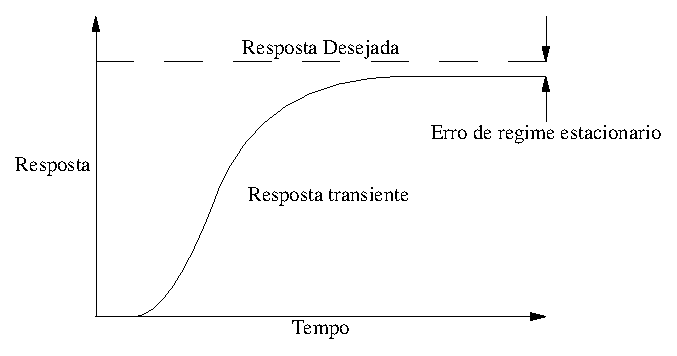
\includegraphics[scale=1]{./pic/C400grafico.eps}
\caption{Gráfico da função Resposta}
\label{fig:funcaoResposta}
\end{figure}

Para realizar o controle de um sistema é necessário que estejam bem definidos os seus requisitos, que são os objetivos a serem atendidos. Quando um sistema por si só já atende aos requisitos, não há a necessidade de controle. De forma oposta, é projetado o sistema de controle, que pode ser em malha aberta ou fechada, clássico ou moderno dependendo das características físicas do sistema. 

Para a execução de um sistema de controle podem ser verificados requisitos do sistema de duas formas básicas, sendo a primeira através dos testes e levantamento empírico da sua curva de resposta ou através de seu modelo matemático, quando trabalha-se com elementos já bem estudados e com a equação que representa seu comportamento empírico bem estabelecida por diversos estudos anteriores.



\newpage



%%%%%%%%%%%%%%%%%%%%%%%%%%%%%%%%%%%%%%%%%%%%%%%%%%%%%%%%%%%
\section{Controle Moderno Não Convencional \\ Lógica Paraconsistente}
%%%%%%%%%%%%%%%%%%%%%%%%%%%%%%%%%%%%%%%%%%%%%%%%%%%%%%%%%%%

O controle moderno trata de sistemas multivariáveis, não lineares ou variantes no tempo de forma mais apropriada do que o controle clássico, reduzindo a complexidade das expressões para que haja a possibilidade de um processamento satisfatório.
Dentro do universo do controle moderno, existe ainda o controle convencional que utiliza a análise de sistemas de controle no espaço de estados, que utiliza n-equações de primeira ordem combinadas em uma equação diferencial vetor-matricial, de forma a simplificar e possibilitar o trabalho com uma quantidade de variáveis alta sem que haja um grande impacto no processamento.  \cite{Ogata} 
Outra forma de controle moderno é denominada controle não convencional, aonde estão situadas diversas técnicas como controle adaptativo, algoritmos adaptativo e genético, redes neurais, as lógicas Fuzzy e Paraconsistente, que é alvo da abordagem do presente trabalho, entre outras.

A lógica, como ramo filosófico que trata das relações de coerência racional e discursiva, proposições e conclusões, tem como origem a Grécia Antiga com o seu primeiro arranjo formal em \emph{Tópicos} de Aristóteles por volta de 340 a.C. Apesar de suas bases serem conhecidas e discutidas por diversos pensadores anteriores, não havia a formalização de uma teoria bem fundada, apenas o tratamento de ideias como consistência e consequências da contraditoriedade por exemplo. 

Os princípios da lógica enunciadas por Aristóteles são basilares para a teoria clássica e moldaram o pensamento e a noção de consistência, ou não contraditoriedade, estreitamente conectadas ao conceito de completude e podem ser descritos formalmente assim:


\begin{enumerate}
\item Princípio de Identidade: 
    \begin{math}
	A \rightarrow B 
	\textrm{ ou } 
	\forall x(x=x);
    \end{math}

\item Princípio do Terceiro Excluído:
    \begin{math}
	A \vee \neg A
	\textrm{ ou }
	\forall x(Ax \vee \neg Ax);
    \end{math}

\item Princípio da Não Contradição: 
    \begin{math}
	\neg (A \wedge \neg A)
	\textrm{ ou }
	\forall x\neg(Ax \wedge \neg Ax).
    \end{math}

\end{enumerate}

O grande desenvolvimento da lógica, principalmente nos séculos XIX e XX, forneceu ferramental para caracterização e tratamento preciso da lógica clássica e também possibilitou o desenvolvimento de sistemas lógicos não clássicos, possibilitando rearranjos, experimentações e questionamentos de dogmas secularmente estabelecidos.

Uma questão que já havia sido objeto de estudo por diversos pensadores desde os pré-socráticos, como Heráclito e sua doutrina da harmonia dos opostos, é a questão da contradição, que por vezes incomodou-os mas que nunca havia sofrido um tratamento formal como o desenvolvido por Newton C. A. da Costa(1929- ) e Stanislaw Jaskiwski(1906-1965), que propuseram e desenvolveram sistemas lógicos que fossem capazes de lidar com essas inconsistências. 

Para (da Costa e Marconi, 1989), ao restringir em um certo sistema lógico o princípio da não contradição, obtém-se um resultado que pertence à lógica denominada Paraconsistente.


Assim sendo, para uma dada teoria, se houver um símbolo de negação, como por exemplo "\emph{$\neg $}", se em qualquer fórmula fechada \emph{A} não for demonstrável \emph{$A$} e \emph{$\neg A $} a teoria é consistente (não contraditória), senão, ela é inconsistente(contraditória).


Teoria é definida por (Evandro Luís Gomes, 2013 p.4) como sendo:
\citacao
{
...um conjunto de fórmulas(expressões bem formuladas) de uma linguagem, fechadas por uma determinada relação de consequência, que caracteriza a lógica subjacente à teoria, da qual ela herda todas as suas características estruturais como, por exemplo, consistência(não contraditoriedade) e completude.
}

Na lógica clássica, uma teoria é completa, se e somente se, for consistente para toda a fórmula fechada \emph{A} onde \emph{A} e \emph{$\neg A$} é teorema da teoria e a teoria é trivial ou supercompleta se todas as fórmulas expressáveis forem demonstráveis, tanto \emph{A} quanto \emph{$ \neg A$}.


Sendo que toda a lógica paraconsistente, não se pode deduzir qualquer fórmula à partir de uma fórmula \emph{A} e sua negação \emph{$\neg A$}, mostrando assim que as noções de inconsistência (contraditoriedade) e trivialidade são de fato independentes.



%A lógica paraconsistente, segundo (Evandro Luis Gomes, 2013) 
%"Apesa do problema da existência de contradições aceitáveis já vir chamando a atenção de lógicos e filósofos pelo menos desde o tempo de Aristóteles, até o aparecimento das lógicas paraconsistentes não se dispunha de um aparato lógico para o estudo das contradiçẽos." 
%Arruda(1990, p.5-6) in Evandro Luis Gomes, 2013 p.5

%"E, como da Costa mesmo reconhecera antes, em 1958, a não trivialidade é que é decisiva ao exercício teórico-racional."
%Evandro Luis Gomes, 2013 p.439



%%%%%%%%%%%%%%%%%%%%%%%%%%%%%%%%%%%%%%%%%%%%%%%%%%%%%%%%%%%%
\subsection{Reticulado de Hasse}
%%%%%%%%%%%%%%%%%%%%%%%%%%%%%%%%%%%%%%%%%%%%%%%%%%%%%%%%%%%%

A lógica paraconsistente sendo apropriada para tratar dados inconsistentes foi utilizada em 1987, por H. Blair e V. S. Subrahmanian para representar e codificar o funcionamento de bancos de dados inconsistentes. Pouco depois Costa, Subrahmanian e Vago propuseram a lógica paraconsistente anotada e sua extensão a uma lógica de predicados paraconsistente anotada de primeira ordem. 

Nas lógicas paraconsistentes anotadas, uma proposição $P$ utiliza um reticulado formado por pares ordenados tal que: 

\begin{center}
\begin{equation}
\tau = \{ ( \mu , \lambda ) \mid \mu ,\lambda \in [0,1] \subset \Re \}
\end{equation}
\end{center}

de acordo com graus de cresça das constantes anotacionais do reticulado de Hasse, associado à Lógica Paraconsistente Anotada com anotação de dois valores (LPA2v), formalmente descritas como 

\begin{center}
\begin{equation}
  \tau = \{ \top , V, F, \bot \}
\end{equation}
\end{center}

os quais descrevem os extremos do reticulado como sendo inconsistente, verdadeiro, falso e paracompleto, respectivamente. 

\begin{figure}[!htb]
\center\includegraphics{./pic/C421reticuladoHasse.eps}
\caption{Reticulado finito de Hasse}
\label{fig:reticuladoHasse}
\end{figure}

Para toda proposição $P$ há um par de valores, chamada de anotação, $(\mu , \lambda )$, onde $\mu$ é o grau de evidência favorável e $\lambda $ é o grau de evidência desfavorável, representada como  $P_{( \mu , \lambda )}$ .

%$P_{( \mu , \lambda )}$
Como exemplificação, para uma proposição $P \equiv$ \emph{"A temperatura do aquecedor atingiu o valor desejado."}, assume-se dois especialistas para realizarem a leitura dos valores da anotação. Em um sistema físico, os especialistas geralmente são sensores, como neste caso, poderiam ser sensores de temperatura.

\begin{itemize}
\item 
$\mu$ = grau de evidência favorável (especialista 1), ou seja, com quanto de certeza, em um intervalo fechado $[0,1]$, sendo 0 para grau nulo de certeza e 1 grau máximo de certeza para a dada proposição $P$;

\item
$\lambda$ = grau de evidência desfavorável (especialista 2), ou seja, com quanto de certeza, em um intervalo fechado $[0,1]$, sendo 0 o grau nulo de certeza à evidência desfavorável e 1 o grau máximo de certeza à evidência desfavorável para a dada proposição $P$.

\end{itemize}


Assim, podemos interpretar da seguinte forma os valores da anotação para as posições extremas do reticulado finito de Hasse:

\begin{itemize}
\item 
$(\mu, \lambda ) = (1,0)$ : Há um grau de evidência favorável total e um grau de evidencia desfavorável nulo, ou seja, a afirmação da proposição é máxima e sua negação é nula, assim,  $P$ é \emph{Verdadeira} e \emph{A temperatura do aquecedor atingiu o valor desejado};

\item 
$(\mu, \lambda ) = (0,1)$ : Há um grau de evidência favorável nulo e um grau de evidencia desfavorável máximo, ou seja, a afirmação da proposição é nula e sua negação é máxima, assim,  $P$ é \emph{Falsa} e \emph{A temperatura do aquecedor não atingiu o valor desejado};

\item 
$(\mu, \lambda ) = (1,1)$ : Há um grau de evidência favorável máximo e também um grau de evidencia desfavorável máximo, ou seja, a afirmação da proposição é máxima e sua negação também é máxima, assim,  $P$ é \emph{Inconsistente} e \emph{A temperatura do aquecedor atingiu e não atigiu o valor desejado}, contradição;

\item 
$(\mu, \lambda ) = (0,0)$ : Há um grau de evidência favorável nulo e também um grau de evidencia desfavorável nulo, ou seja, a afirmação da proposição é nula e sua negação também é nula, assim,  $P$ é \emph{Indeterminada} e \emph{A temperatura do aquecedor nem atingiu o valor desejado e nem não atingiu o valor desejado}, situação paracompleta.

\end{itemize}

Os graus de evidência podem assumir valores não extremos:

\begin{itemize}
\item 
$(\mu, \lambda ) = (0.8,0.3)$ : Crê-se com grau de evidência favorável de 80\% e um grau de evidencia desfavorável de 30\%  que \emph{A temperatura do aquecedor atingiu do valor desejado}.
\end{itemize}

Existe um operador de negação ($\sim $) sobre $\tau$ de forma que :
\begin{center}
\begin{equation}
\sim  : \mid \tau \mid \rightarrow \mid \tau , \sim(\mu, \lambda ) = (\lambda, \mu )
\end{equation}
\end{center}

Então,
\begin{center}
\begin{equation}
P_{(0.8,0.3)} \leftrightarrow \textrm{"   "} \sim P_{(0.3,0.8)}
\end{equation}
\end{center}

\begin{itemize}
\item 
$(\mu, \lambda ) = (0.8,0.3) = \sim (0.3,0.8)$ : Não crê-se que há um grau de evidência favorável de 30\% e um grau de evidencia desfavorável de 80\% que \emph{A temperatura do aquecedor atingiu do valor desejado}.
\end{itemize}



%%%%%%%%%%%%%%%%%%%%%%%%%%%%%%%%%%%%%%%%%%%%%%%%%%%%%%%%%%%%
\subsection{Quadrado Unitário no Plano Cartesiano - QUPC}
%%%%%%%%%%%%%%%%%%%%%%%%%%%%%%%%%%%%%%%%%%%%%%%%%%%%%%%%%%%%

Uma outra forma de representação da anotação é utilizando o Quadrado Unitário no Plano Cartesiano (QUPC) no qual são transpostos os pontos extremos às respectivas posições de acordo com o par ordenado,  $(\mu, \lambda ) \leftrightarrow (x,y) $, assim o eixo $x$ corresponde ao grau de evidência favorável e o eixo $y$ corresponde ao grau de evidência desfavorável, conforme mostrado na Figura \ref{fig:reticuladoQUPC}.



\begin{figure}[!htb]
\center\includegraphics{./pic/C422qupc.eps}
\caption{Representação do reticulado no quadrado unitário no plano cartesiano}
\label{fig:reticuladoQUPC}
\end{figure}

Os pontos extremos assim representam:

\begin{itemize}
\item $A: (0,0) = \bot \Rightarrow $ Paracompleto;
\item $B: (0,1) = F \Rightarrow $ Falso;
\item $C: (1,1) = \top \Rightarrow $ Contradição;
\item $D: (1,0) = V \Rightarrow $ Verdade.
\end{itemize}

O segmento de reta $\overline{BD}$, entre os pontos referentes às condições $Verdade$ e $Falso$, conforme mostrado na Figura \ref{fig:retaPerfeitamenteDefinida}, é denominada de \emph{Reta Perfeitamente Definida} e dada uma anotação $(\mu, \lambda )$ situada nela, a soma das evidências anotadas é sempre o valor unitário do quadro. 

\begin{figure}[!htb]
\center\includegraphics{./pic/C424retaPerfeitamenteDefinida.eps}
\caption{Representação da Reta Perfeitamente Definida}
\label{fig:retaPerfeitamenteDefinida}
\end{figure}

A relação dos graus de evidência da anotação quando coincidente à Reta Perfeitamente Definida é: 

\begin{center}
\begin{equation}
\mu + \lambda = 1
\label{eq:evidenciaUnitaria1}
\end{equation}
\end{center}

Assim, temos que:

\begin{center}
\begin{equation}
\mu + \lambda - 1 = 0
\label{eq:evidenciaUnitaria}
\end{equation}
\end{center}


Os graus de evidência não precisam apresentar valores complementares, possuem independência entre si, assim das Equações  
\ref{eq:evidenciaUnitaria1} e 
\ref{eq:evidenciaUnitaria} 
é elaborado o conceito de 
\emph{Grau de Contradição}($G_{ct}$), 
assim temos: 

\begin{center}
\begin{equation}
G _{ct} = \mu + \lambda - 1
\label{eq:grauIncerteza}
\end{equation}
\end{center}

quanto mais próximo da Reta Perfeitamente Definida, menor o grau de contradição apresentado pelos graus de evidência. 
Quanto mais afastado da Reta Perfeitamente Definida estiver o ponto, e mais próximo aos pontos A ou C, maior é o grau de contradição. 

Quando a anotação estiver situada na região entre os pontos BCD, acima da reta perfeitamente definida, o grau de contradição é denominado 
\emph{Grau de Inconsistência} ($G_{it}$), 
e isso ocorre quando, $\mu \ge \lambda $, de forma oposta, quando $\mu < \lambda $ a anotação está situada na região entre os pontos BAD, abaixo da reta perfeitamente definida, e o grau de contradição é denominado 
\emph{Grau de Indefinição} ($G_{id}$), 
então pode-se dizer que:

\begin{center}
\begin{equation}
-1 \le G _{id}  <  0 \le G _{it} \le 1
\label{eq:grauInconsistenciaIndefinicao}
\end{equation}
\end{center}
e
\begin{center}
\begin{equation}
-1 \le G _{ct} \le 1
\label{eq:grauInconsistenciaIndefinicao1}
\end{equation}
\end{center}


O segmento de reta $\overline{ AC }$ , entre os pontos referentes às condições \emph{Paracompleto} e \emph{Contradição}, conforme mostrado na Figura \ref{fig:retaPerfeitamenteIndefinida}, é denominada de \emph{Reta Perfeitamente Indefinida} e dada uma anotação $(\mu, \lambda )$ situada nela, a subtração das evidências anotadas é sempre zero, $\mu = \lambda$, e de forma contrária, quando a anotação está posicionada de forma não coincidente à Reta Perfeitamente Indeterminada, significa que $\mu \neq \lambda$.

\begin{figure}[!htb]
\center\includegraphics{./pic/C426retaPerfeitamenteIndefinida.eps}
\caption{Representação da Reta Perfeitamente Indefinida}
\label{fig:retaPerfeitamenteIndefinida}
\end{figure}

A relação dos graus de evidência para uma anotação cuja posição coincide com a Reta Perfeitamente Indefinida é: 

\begin{center}
\begin{equation}
\mu - \lambda = 0
\label{eq:evidenciaIndefinida}
\end{equation}
\end{center}

De forma análoga ao Grau de contradição, da Equação \ref{eq:evidenciaIndefinida} é elaborado o conceito de \emph{Grau de Certeza} ($G _c$), assim temos que: 

\begin{center}
\begin{equation}
G _{c} = \mu - \lambda
\label{eq:grauCerteza}
\end{equation}
\end{center}

Quando os graus de evidência, favorável e desfavorável, são iguais, não há certeza em relação à proposição, mas quando são diferentes, alguma certeza pode ser inferida, até a condição máxima onde uma das evidências é total (1) e a outra é nula (0), caracterizando a condição verdadeira ou falsa, afastando o ponto anotado da Reta Perfeitamente Indefinida. 

Quando a anotação situa-se entre os pontos ABC do QUPC, o grau de certeza é denominado \emph{Grau de Falsidade ($G _f$)}, e tal condição ocorre quando $\mu < \lambda $, caso contrário, se $\mu \ge \lambda $, a anotação situa-se entre os pontos ACD do QUPC, e o grau de certeza é denominado \emph{Grau de Verdade ($G _v)$}, então pode-se dizer que:

\begin{center}
\begin{equation}
-1 \le G _{f}  <  0 \le G _{v} \le 1
\label{eq:grauVerdadeFalsidade}
\end{equation}
\end{center}
e
\begin{center}
\begin{equation}
-1 \le G _{c} \le 1
\label{eq:grauCertezaIntervalo}
\end{equation}
\end{center}


Graficamente são representadas como mostra a Figura \ref{fig:retasgcgct}:

\begin{figure}[!htb]
\center\includegraphics{./pic/C428retasgcgct.eps}
\caption{Representação dos Graus de Certeza e Contradição em um plano cartesiano}
\label{fig:retasgcgct}
\end{figure}

A representação ainda é dividia em algumas partes, dependendo da aplicação, estabelecendo quais são os limites que definem cada estado, Verdadeiro, Falso, Paracompleto, Contradição e outros mais que forem pertinentes à aplicação, estão representados pelas linhas tracejadas na Figura \ref{fig:valorControle} e são definidos como:

\begin{itemize}
\item \emph{V $_{scc}$ : Valor limite superior de Controle de Certeza};
\item \emph{V $_{icc}$ : Valor limite inferior de Controle de Certeza};
\item \emph{V $_{sci}$ : Valor limite superior de Controle de Incerteza};
\item \emph{V $_{sci}$ : Valor limite inferior de Controle de Incerteza}.

\end{itemize}

\begin{figure}[!htb]
\center\includegraphics{./pic/C429valorControle.eps}
\caption{Representação dos valores de controle}
\label{fig:valorControle}
\end{figure}

Uma divisão em 12 partes é mostrada na Figura \ref{fig:reticuladoLPA2v} com seus respectivos estados intermediários definidos conforme \cite{JoaoInacio}, sendo 4 regiões extremas:


\begin{figure}[!htb]
\center\includegraphics{./pic/C430gcgct.eps}
\caption{Representação do reticulado da LPA2v subdividido em 12 regiões}
\label{fig:reticuladoLPA2v}
\end{figure}


\begin{itemize}
\item V : Verdadeiro;
\item F : Falso;
\item $\top$ : Contradição;
\item $\bot$ : Paracompleto.
\end{itemize}
e 8 regiões intermediárias: 
\begin{itemize}
\item Qv $\rightarrow  \top$ : Quase Verdade tendendo à Contradição;
\item Qv $\rightarrow  \bot$ : Quase Verdade tendendo à  Paracompleto;
\item Qf $\rightarrow  \top$ : Quase Falso tendendo à Contradição;
\item Qf $\rightarrow  \bot$ : Quase Falso tendendo à Paracompleto;
\item $\top \rightarrow $ f : Contradição tendendo à Falso;
\item $\top \rightarrow $ v : Contradição tendendo à Verdadeiro;
\item $\bot \rightarrow $ f : Paracompleto tendendo à Falso;
\item $\bot \rightarrow $ v : Paracompleto tendendo à Verdadeiro.

\end{itemize}

O reticulado subdividido em 12 regiões como mostrado, é aplicado em situações nas quais a tomada de decisão utiliza estados discretos bem definidos para atuação, onde para cada posição da anotação e respectivamente um estado do reticulado, uma ação é tomada, assim sendo, a quantidade de subdivisões está fortemente dependente da aplicação.



%%%%%%%%%%%%%%%%%%%%%%%%%%%%%%%%%%%%%%%%%%%%%%%%%%%%%%%%%%%%
\subsection{A LPA2v aplicada em Controle}
%%%%%%%%%%%%%%%%%%%%%%%%%%%%%%%%%%%%%%%%%%%%%%%%%%%%%%%%%%%%

A LPA2v aplicada em sistemas de controle utiliza além dos conceitos já estabelecidos, duas outras definições para sua implementação e são elas o \emph{ Grau de Certeza Real ($G _{CR}$)} e o \emph{Grau de Evidência Real ($\mu _{ER}$)} além de trabalhar alguns conceitos básicos de geometria, e pelo fato de possuir uma resolução simples do ponto de vista matemático, motiva este trabalho pela sua implementação eficaz com relação ao controle clássico que exige uma matemática elaborada, dificultando sua implementação em dispositivos de baixo custo e que não possuem hardware específico de processamento de sinais. 


Para a implementação do sistema de controle paraconsistente, primeiramente é necessário que seja definida a proposição que será a base para as análises e tomadas de decisões.

\begin{center}
$ P \equiv $ 
\emph{"A temperatura do aquecedor atingiu o valor desejado."}
\end{center}

Para trabalhar com essa proposição são necessárias pelo menos duas variáveis, sendo uma delas com o valor de temperatura desejada e outra com o valor atual de temperatura. Essas duas variáveis são representadas por meio de duas anotações, mas que antes precisam ser normalizadas. 

\textbf{Variável 1:} 
Valor desejado ou Set point = 37 $^{\circ}$C. 

\begin{equation}
( \mu _{d}, \lambda _{d} ) = (1,0)
\label{eq:setpoint}
\end{equation}

Sendo:

$\mu _{d}$ : grau de evidência favorável ao valor desejado. 

$\lambda _{d}$ : grau de evidência desfavorável ao valor desejado.

Quando o aquecedor atingir a temperatura de 37 $^{\circ}$C, 
crê-se com grau de evidência favorável máxima e grau de evidência desfavorável mínima que a proposição \emph{P} é verdadeira, como mostrado na Equação \ref{eq:setpoint}.



\textbf{Variável 2:} 
Valor de temperatura atual lido pelo sensor: 20 $^{\circ}$C no início do processo.

Supondo, hipoteticamente para facilitar o entendimento, um sensor com range de operação entre 0 e 100 $^{\circ}$C que será lido, linearmente no intervalo de 0 a 10V e normalizado para o intervalo fechado [0,1]. Assim são calculados os graus de evidência:

\begin{equation}
\mu _{a} = 
\frac{Ta - Tmin}{Td - Tmin}
\label{eq:miatual}
\end{equation}

Sendo:

$\mu _{a}$ : Grau de evidência favorável para a leitura da temperatura atual;

\emph{Ta :} Temperatura atual lida pelo sensor;

\emph{Tmin :} Temperatura mínima de leitura pelo sensor de temperatura. Nesse caso, 0 $^{\circ}$C;

\emph{Td :} Temperatura desejada que o aquecedor alcance, estabelecida em 37 $^{\circ}$C.

A normalização pode ser realizada diretamente, desde que todas as variáves da Equação \ref{eq:miatual} estejam na mesma grandeza e na mesma escala, assim os graus de evidência não apresentam dimensão.

Substituindo as variáveis em \ref{eq:miatual}:

\begin{equation}
\mu _{a} = 
\frac{20 - 0}{37 - 0} = 0,54
\label{eq:miatualnumeros}
\end{equation}

Para o valor de $\mu _{a}$ da Equação \ref{eq:miatualnumeros} podemos afirmar que \emph{crê-se com grau de evidência favorável que foi atingido 54\% do percurso para a proposição ser verdadeira.} Como se pode ver, a temperatura inicial proposta foi de 20$^{\circ}$C que é pouco mais da metade da temperatura desejada de 37$^{\circ}$C, caso seja alterada a temperatura desejada para 50$^{\circ}$C, o valor de $\mu _{d}$ seria de 0,4, ou seja, a variável atual seria 40 \% do valor desejado. 

Calculando o grau de evidência desfavorável:

\begin{equation}
\lambda _{a}= 1 - \mu _{a}
\label{eq:lambdaatual}
\end{equation}

Substituindo as variáveis:

\begin{equation}
\lambda _{a}= 1 - 0,54 = 0,46
\label{eq:lambdaatualnumeros}
\end{equation}

O que resulta em uma anotação para a leitura de temperatura atual de: 

\begin{equation}
( \mu _{a}, \lambda _{a} ) = (0,54 , 0,46)
\label{eq:valoratual}
\end{equation}

Calcula-se então o Grau de Contradição (Equação \ref{eq:grauIncerteza} ) e o Grau de Certeza (Equação \ref{eq:grauCerteza}) cruzando os dados das anotações da seguinte forma:

\begin{equation}
G _{ct} = \mu _{d} + \lambda _{a} - 1
\label{eq:grauContradicaoCruzado}
\end{equation}

\begin{equation}
G _{c} = \mu _{d} - \lambda _{a}
\label{eq:grauCertezaCruzado}
\end{equation}


Substituindo (\ref{eq:miatualnumeros}) e (\ref{eq:lambdaatualnumeros}) em (\ref{eq:grauContradicaoCruzado}):

\begin{equation}
G _{ct} = 1 + 0,46 - 1 = 0,46
\label{eq:grauContradicaoResulta}
\end{equation}

Substituindo (\ref{eq:miatualnumeros}) e (\ref{eq:lambdaatualnumeros}) em (\ref{eq:grauCertezaCruzado}):

\begin{equation}
G _{c} = 1 - 0,46 = 0,54
\label{eq:grauCertezaResulta}
\end{equation}

Graficamente pode ser representado como na Figura \ref{fig:gcgctExemplo}.

\begin{figure}[!htb]
\center\includegraphics{./pic/C440gcgctExemplo.eps}
\caption{Representação de Gc = 0.54 e Gct = 0.46}
\label{fig:gcgctExemplo}
\end{figure}



%%%%%%%%%%%%%%%%%%%%%%%%%%%%%%%%%%%%%%%%%%%%%%%%%%%%%%%%%%%%
%%%%%%%%%%%%%%%%%%%%%%%%%%%%%%%%%%%%%%%%%%%%%%%%%%%%%%%%%%%%



\chapter{Sistema eletrônico}
\section{Controlador}
\section{Drive}
\section{Aquecedor}
\subsection{ Temperatura }
A temperatura regula diversas propriedades físicas, químicas e biológicas como o caso do corpo humano, reações catalíticas, maturação fetal. Pode ser definida tanto no nível macroscópico, pela sensação de quente e frio, quanto no nível microscópico através do grau de agitação das moléculas. É uma propriedade intensiva de um sistema, ou seja, não depende da massa, assim como a viscosidade, pressão e densidade, contrapondo-se à propriedade extensiva como a própria massa, o volume, a energia cinética e a quantidade de movimento.
A temperatura governa o processo de transferência de energia térmica, calor, entre os corpos. Assim diz-se que quando há um equilíbrio térmico, há uma igualdade de temperatura.

\subsection{ Unidade de Temperatura }
O Sistema Internacional de Unidades através da 10ª Comissão Geral de Pesos e Medidas (CGPM, 1954) define a unidade de temperatura como sendo $\frac{1}{273,16} $  do ponto triplo da água\footnote{Ponto de equilíbrio entre temperatura, pressão e volume aonde a água pode coexistir nos estados sólido, líquido e gasoso.}. E na 13ª CGPM adota o nome kelvin, e K como símbolo padrão para temperatura.
Isso significa que a temperatura do ponto tríplo da água é:
\[ 273,16 \ kelvins \   ou T_{tpw} = 273,16 K \]

Como modo prático, é adotado o símbolo T e $ T_0 = 273.15K $ como temperatura de fusão da água. Assim para um dado valor de temperatura na escala kelvin tem-se que:
\[t = T - T_0\]
Sendo \emph{t} a temperatura em graus Celsius, com símbolo \textcelsius. Ambas as unidades de medida de temperatura, kelvin e graus Celsius, são unidades da Escala Internacional de Temperatura (International Temperature Scale) de 1990.
A conversão entre ambas as unidades é:
\[ t[ ^o C ] = T[K] - 273,15 \]

Ambas as escalas são ditas centígradas por possuírem cem divisões entre seus pontos de referência, fusão e ebulição da água.

Os pontos de referência são adotados a partir de condições estáveis de determinados sistemas, ou substâncias, para garantir uma uniformidade e a possibilidade de aferição dos instrumentos de medição.



\section{Sensores}
\section{Programação}
\subsection{Linguagem}
\subsection{Compilador}
\subsection{Técnicas de Programação}



\chapter{Apresentação e discussão dos resultados}

\section{ A construção do sistema de controle }	

A construção dos sistema de controle possui de um modo geral três grandes etapas, sendo a primeira o momento de estabelecimento dos objetivos, das variáveis de controle e especificações do sistema. Em um segundo momento é estabelecida a configuração do sistema e é gerado um modelo do sistema a partir dos modelos de suas partes. Finalmente é feito o desenvolvimento do controle do sistema, simulação e análise. Caso o sistema ainda não atenda os requisitos, uma nova interação deve ser executada partindo do segundo momento.

\subsection{ Estabelecer os objetivos do controle }

Mostrar o comportamento do sistema sem controle.

Gráficos de comportamento atual x comportamento desejado

\subsection{ Identificar a variável a ser controlada }
\subsection{ Escrever as especificações }
\subsection{ Estabelecer a configuração do sistema }
\subsection{ Obter um modelo do processo e suas partes }
\subsection{ Descrever o controlador e parâmetros de ajuste }
\subsection{ Otimizar parâmetros e analisar performance }




\chapter{Considerações Finais - Conclusão}


\citacao{
 typesetting systems: \LaTeX{}
}



%%-------------------------------------- Bibliografia

\bibliographystyle{apa}
\bibliography{bibliografia.bib}


%%-------------------------------------- Apendice
%%\appendix
%%\chapter{Titulo do Apendice}

%%-------------------------------------- Anexo
%%\annex
%%\chapter{Titulo do Anexo}



\end{document}




% bibliographystyle tipos
%http://www.cs.stir.ac.uk/~kjt/software/latex/showbst.html

%%%% Estrutura base do arquivo
%%[] http://www.demat.ufma.br/monografia.php <acesso em 12/10/2015>
%%%% Inclusão de pacote de acentuação Francês/Portugues
%%[] https://www.overleaf.com/help/61-how-do-i-do-to-use-letters-with-accents-e-dot-g-in-french-or-portuguese#.Vhwirc8Tr18 <acesso em 12/10/2015 


%http://link.periodicos.capes.gov.br/sfxlcl41?frbrVersion=2&ctx_ver=Z39.88-2004&ctx_enc=info:ofi/enc:UTF-8&ctx_tim=2015-10-27T23%3A55%3A45IST&url_ver=Z39.88-2004&url_ctx_fmt=infofi/fmt:kev:mtx:ctx&rfr_id=info:sid/primo.exlibrisgroup.com:primo3-Article-doaj&rft_val_fmt=info:ofi/fmt:kev:mtx:journal&rft.genre=article&rft.atitle=Implementation+of+PID+and+Fuzzy+PID+controllers+for+Temperature+control+in+CSTR&rft.jtitle=International+Journal+of+Advanced+Research+in+Computer+Science&rft.btitle=&rft.aulast=&rft.auinit=&rft.auinit1=&rft.auinitm=&rft.ausuffix=&rft.au=S.+Srinivasulu+Raju&rft.aucorp=&rft.date=20130501&rft.volume=04&rft.issue=05&rft.part=&rft.quarter=&rft.ssn=&rft.spage=12&rft.epage=&rft.pages=&rft.artnum=&rft.issn=0976-5697&rft.eissn=&rft.isbn=&rft.sici=&rft.coden=&rft_id=info:doi/&rft.object_id=&svc_val_fmt=info:ofi/fmt:kev:mtx:sch_svc&rft.eisbn=&rft_dat=%3Cdoaj%3E01c00f89709d40549e219bbc941a6a0a%3C/doaj%3E%3Cgrp_id%3E7778711627802309381%3C/grp_id%3E%3Coa%3E%3C/oa%3E&rft_id=info:oai/&svc.fulltext=yes&req.language=por

% http://link.periodicos.capes.gov.br/sfxlcl41?frbrVersion=3&ctx_ver=Z39.88-2004&ctx_enc=info:ofi/enc:UTF-8&ctx_tim=2015-10-27T23%3A55%3A45IST&url_ver=Z39.88-2004&url_ctx_fmt=infofi/fmt:kev:mtx:ctx&rfr_id=info:sid/primo.exlibrisgroup.com:primo3-Article-springer_jour&rft_val_fmt=info:ofi/fmt:kev:mtx:&rft.genre=&rft.atitle=Adaptive+fuzzy+tuning+of+PID+controllers&rft.jtitle=Neural+Computing+and+Applications&rft.btitle=&rft.aulast=Esfandyari&rft.auinit=&rft.auinit1=&rft.auinitm=&rft.ausuffix=&rft.au=Esfandyari%2C+Morteza&rft.aucorp=&rft.date=201312&rft.volume=23&rft.issue=1&rft.part=&rft.quarter=&rft.ssn=&rft.spage=19&rft.epage=28&rft.pages=&rft.artnum=&rft.issn=0941-0643&rft.eissn=1433-3058&rft.isbn=&rft.sici=&rft.coden=&rft_id=info:doi/10.1007%2Fs00521-012-1215-8&rft.object_id=&svc_val_fmt=info:ofi/fmt:kev:mtx:sch_svc&rft.eisbn=&rft_dat=%3Cspringer_jour%3E10.1007%2Fs00521-012-1215-8%3C/springer_jour%3E%3Cgrp_id%3E6653138538760267648%3C/grp_id%3E%3Coa%3E%3C/oa%3E&rft_id=info:oai/&svc.fulltext=yes&req.language=por

%http://link.periodicos.capes.gov.br/sfxlcl41?frbrVersion=2&ctx_ver=Z39.88-2004&ctx_enc=info:ofi/enc:UTF-8&ctx_tim=2015-10-27T23%3A55%3A45IST&url_ver=Z39.88-2004&url_ctx_fmt=infofi/fmt:kev:mtx:ctx&rfr_id=info:sid/primo.exlibrisgroup.com:primo3-Article-sciversesciencedirect_elsevier&rft_val_fmt=info:ofi/fmt:kev:mtx:&rft.genre=article&rft.atitle=A+multivariable+predictive+fuzzy+PID+control+system&rft.jtitle=Applied+Soft+Computing+Journal&rft.btitle=&rft.aulast=Savran&rft.auinit=&rft.auinit1=&rft.auinitm=&rft.ausuffix=&rft.au=Savran%2C+Aydogan&rft.aucorp=&rft.date=2012&rft.volume=&rft.issue=&rft.part=&rft.quarter=&rft.ssn=&rft.spage=&rft.epage=&rft.pages=&rft.artnum=&rft.issn=1568-4946&rft.eissn=&rft.isbn=&rft.sici=&rft.coden=&rft_id=info:doi/10.1016%2Fj.asoc.2012.11.021&rft.object_id=&svc_val_fmt=info:ofi/fmt:kev:mtx:sch_svc&rft.eisbn=&rft_dat=%3Csciversesciencedirect_elsevier%3ES1568-4946%2812%2900505-4%3C/sciversesciencedirect_elsevier%3E%3Cgrp_id%3E824269217450252803%3C/grp_id%3E%3Coa%3E%3C/oa%3E&rft_id=info:oai/&svc.fulltext=yes&req.language=por

%http://link.periodicos.capes.gov.br/sfxlcl41?frbrVersion=3&ctx_ver=Z39.88-2004&ctx_enc=info:ofi/enc:UTF-8&ctx_tim=2015-10-27T23%3A55%3A45IST&url_ver=Z39.88-2004&url_ctx_fmt=infofi/fmt:kev:mtx:ctx&rfr_id=info:sid/primo.exlibrisgroup.com:primo3-Article-gale_ofa&rft_val_fmt=info:ofi/fmt:kev:mtx:&rft.genre=article&rft.atitle=A+multivariable+predictive+fuzzy+PID+control+system.&rft.jtitle=Applied+Soft+Computing+Journal&rft.btitle=&rft.aulast=&rft.auinit=&rft.auinit1=&rft.auinitm=&rft.ausuffix=&rft.au=Savran%2C+Aydogan&rft.aucorp=&rft.date=20130501&rft.volume=13&rft.issue=5&rft.part=&rft.quarter=&rft.ssn=&rft.spage=2658&rft.epage=&rft.pages=&rft.artnum=&rft.issn=1568-4946&rft.eissn=&rft.isbn=&rft.sici=&rft.coden=&rft_id=info:doi/&rft.object_id=&svc_val_fmt=info:ofi/fmt:kev:mtx:sch_svc&rft.eisbn=&rft_dat=%3Cgale_ofa%3E339267889%3C/gale_ofa%3E%3Cgrp_id%3E8626435848081561867%3C/grp_id%3E%3Coa%3E%3C/oa%3E&rft_id=info:oai/&svc.fulltext=yes&req.language=por

%http://link.periodicos.capes.gov.br/sfxlcl41?frbrVersion=4&ctx_ver=Z39.88-2004&ctx_enc=info:ofi/enc:UTF-8&ctx_tim=2015-10-27T23%3A57%3A23IST&url_ver=Z39.88-2004&url_ctx_fmt=infofi/fmt:kev:mtx:ctx&rfr_id=info:sid/primo.exlibrisgroup.com:primo3-Article-springer_jour&rft_val_fmt=info:ofi/fmt:kev:mtx:&rft.genre=article&rft.atitle=Neuro+PID+control+of+power+generation+using+a+low+temperature+gap&rft.jtitle=Artificial+Life+and+Robotics&rft.btitle=&rft.aulast=Han&rft.auinit=&rft.auinit1=&rft.auinitm=&rft.ausuffix=&rft.au=Han%2C+Kun-Young&rft.aucorp=&rft.date=201109&rft.volume=16&rft.issue=2&rft.part=&rft.quarter=&rft.ssn=&rft.spage=178&rft.epage=184&rft.pages=&rft.artnum=&rft.issn=1433-5298&rft.eissn=1614-7456&rft.isbn=&rft.sici=&rft.coden=&rft_id=info:doi/10.1007%2Fs10015-011-0913-0&rft.object_id=&svc_val_fmt=info:ofi/fmt:kev:mtx:sch_svc&rft.eisbn=&rft_dat=%3Cspringer_jour%3E10.1007%2Fs10015-011-0913-0%3C/springer_jour%3E%3Cgrp_id%3E5844933895106062701%3C/grp_id%3E%3Coa%3E%3C/oa%3E&rft_id=info:oai/&svc.fulltext=yes&req.language=por



